%Engenharia de Software
%Relatório primeiro sprint
\documentclass[12pt, a4paper, twocolumn]{article}

\usepackage[a4paper,top=2.5cm,bottom=2.554cm,left=2.554cm,right=2.554cm]{geometry}

\usepackage[portuguese]{babel}
\usepackage[utf8]{inputenc}
\usepackage{url}
\usepackage[pdftex]{graphicx}
\graphicspath{{./imagens/}}
\usepackage{color}
\usepackage{indentfirst}
\usepackage{mathtools}
\usepackage{caption}

\title{Relatório do primeiro Sprint\\ \textbf{Python Basics, Expressões Regulares e Manipulação de Arquivos}
		}
\author{Daniel Gomes, Érica Costa, Marcela Malaquias, Paulo Vicktor Felix}

\begin{document}

\maketitle

\begin{abstract}
Neste sprint, o grupo devia aprender:
\begin{itemize}
	\item \textbf{Básicos de python}: suas principais funções e funcionamento da linguagem
	\item \textbf{Expressões Regulares}: busca de padrões em textos e suas correspondências
	\item \textbf{Manipulação de Arquivos}: leitura e criação
\end{itemize}

Além disso, relatar o desenvolvimento do processo de aprendizagem, relacionando-o ao objetivo final do trabalho. Assim, concluir o relatório e fazer \textit{upload} para o Git.

\end{abstract}

\section{Básicos de Python}
Iniciando com funções simples de saída (Figura 1), operações matemáticas (Figura 2) e entrada de dados (Figura 3), buscamos aprender a utilizar as ferramentas disponíveis pela linguagem. Para isso, foram utilizadas video-aulas e livros de programação para que fosse possível agregar o conhecimento de programação.
\begin{figure}[htb!]
	\centering
	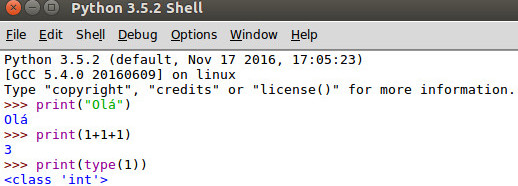
\includegraphics[scale = 0.45]{printss.jpg}
	\caption{Uso da função print() e type().}
\end{figure}
\begin{figure}[htb!]
	\centering
	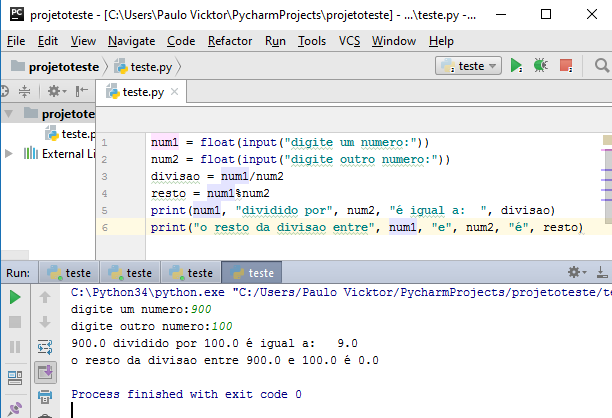
\includegraphics[scale = 0.5] {operadores_matematicos.png}
	\caption{Uso de operadores matemáticos.}
\end{figure}
\begin{figure}[htb!]
	\centering
	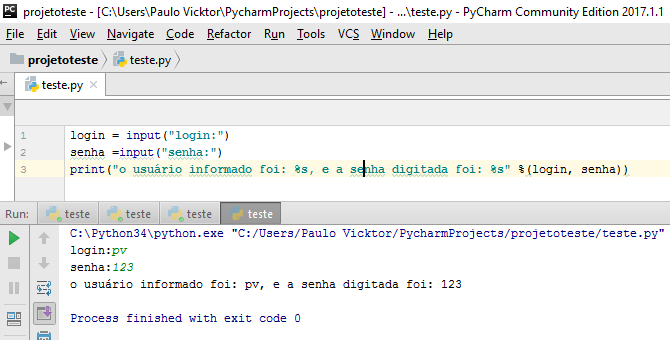
\includegraphics[scale = 0.45] {entrada_dados.png}
	\caption{Uso de entrada de dados.}
\end{figure}

\pagebreak

\section{Expressões Regulares}
Por meio da utilização do livro "Automate the boring stuff with python"[1], conseguimos aprender a criar scripts para reconhecimento de padrões e criar correspondências por esses padrões. Um exemplo prático de aplicação para essa função é criar um programa que identifica se a string digitada corresponde a um email, por meio da quantidade e tipo dos caracteres (Figura 5).
\begin{figure}[htb!]
	\centering
	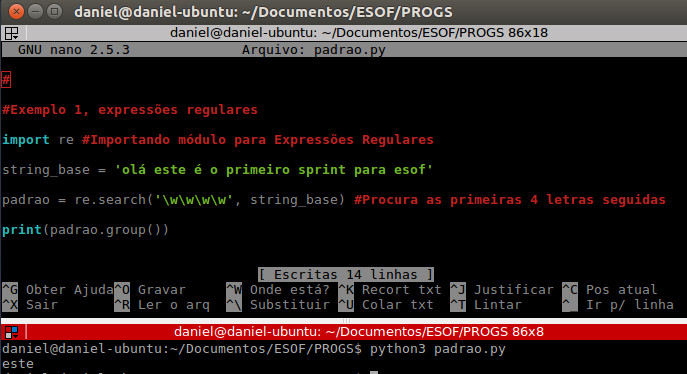
\includegraphics[scale = 0.32] {re1.jpg}
	\caption{Identificação de um padrão}
\end{figure}

\begin{figure}[htb!]
	\centering
	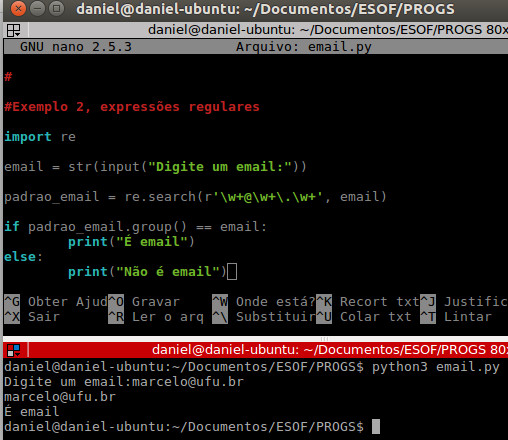
\includegraphics[scale = 0.43] {re2.jpg}
	\caption{Verificar se é email}
\end{figure}

Além disso, é possível categorizar em uma lista, por meio dos padrões observados no texto, como na Figura 6, de modo um pouco mais complexo.

\begin{figure}[htb!]
	\centering
	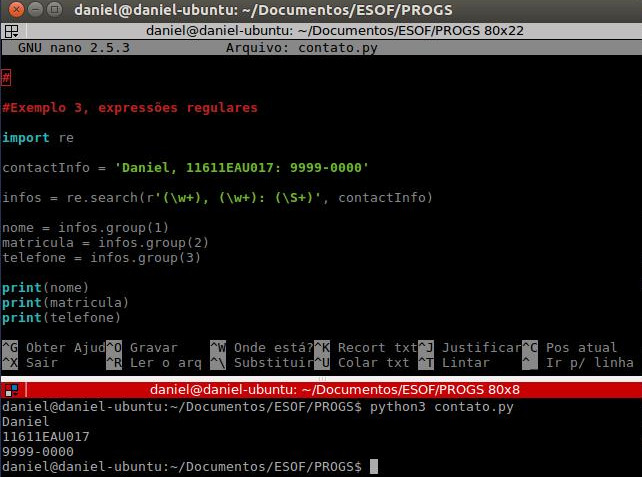
\includegraphics[scale = 0.35] {re3.jpg}
	\caption{Lista de informações}
\end{figure}
\pagebreak
\section{Manipulação de arquivos}
Nesta parte, o grupo ficou responsável de buscar informações sobre como abrir, criar e editar arquivos em python. Para isso, foi utilizado o livro citado anteriormente, e como resultado do estudo, obtivemos alguns programas.

Na Figura 7 foi criado um arquivo, depois editado e lido.
\begin{figure}[htb!]
	\centering
	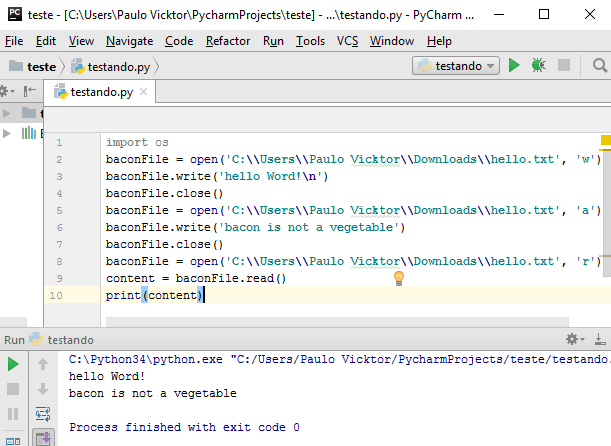
\includegraphics[scale = 0.5] {imagem3.png}
	\caption{Manipulando um arquivo}
\end{figure}
\pagebreak
Já na Figura 8, é criado um arquivo binário de informações, o qual pode ser acessado futuramente. Sendo possível acessar do mesmo programa ou de outro programa a ser desenvolvido.

\begin{figure}[htb!]
	\centering
	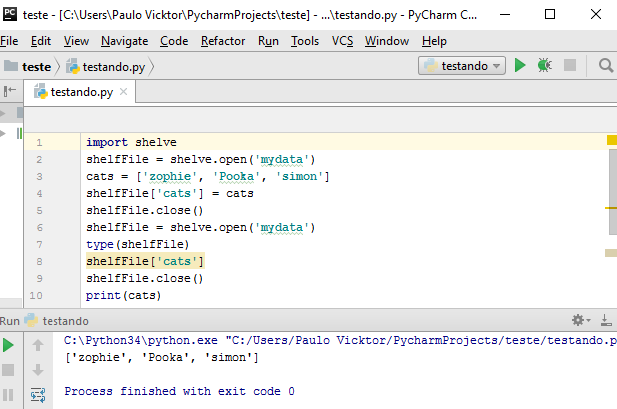
\includegraphics[scale = 0.47] {imagem4.png}
	\caption{Usando módulo Shelve}
\end{figure}

E, finalmente, na Figura 9, é criado um arquivo '.py' que pode ser rodado pelo interpretador e convocado em outro programas.

\begin{figure}[htb!]
	\centering
	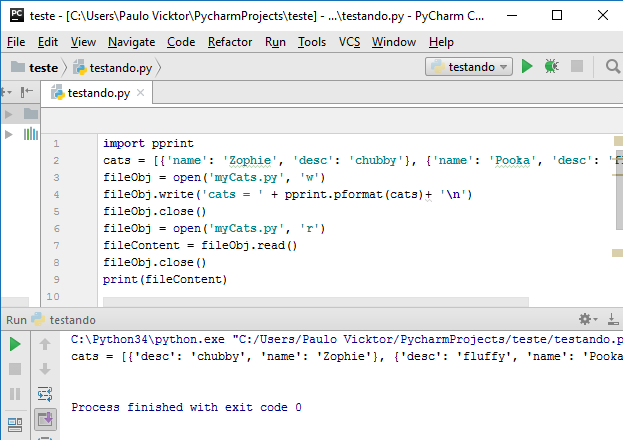
\includegraphics[scale = 0.5] {imagem5.png}
	\caption{Criando '.py'}
\end{figure}

\pagebreak
\section{Referências}
[1] SWEIGART, Al. "Automate the boring stuff with python", 2015. \\

[2] Aula 14 - Expressões Regulares: \url{https://www.youtube.com/watch?v=aPk2ruhi2Zk}. Acesso em 20 de Abril de 2017.



\end{document}
